\section{Version Control}
A version control system (VCS) is essentially a bookkeeping device for software development.
While humans can theoretically achieve this collaboration manually, this amounts to standardizing naming conventions, keeping multiple copies of work, logistical nightmares resulting from simultaneous editing or distributing changes, and resolving conflicts from multiple edits to the same file.
These headaches can all be solved by using a VCS.
One popular VCS is Git, and we recommend using it across the board. It is a free and open-source, distributed VCS. Commonly partnered with Git is GitHub, a cloud-based repository that enables developers to store and manage their code easily. A repository is just a location where code is stored and organized. Using GitHub allows your team to have a single source of truth for your entire codebase. For the remainder of this chapter, we will only discuss using GitHub to setup and manage this repository.

\subsection{Git Basics}
On Mac, as well as some Linux distributions, Git is included with the Operating System. If it is not already installed on your system, you will need to download and install it.

On Mac or Linux, you can open a program called \textit{Terminal} that allows you to run commands. From your terminal, type \pythoninline{git --version} to verify installation.
To install Git on Windows, follow the installation instructions for GitHub Desktop.

To get started, create a GitHub account. After this is done, create a new repository in GitHub called \texttt{test\textunderscore repository}. You should now have a reference URL for this new repository at:\\ \pythoninline{https://github.com/<your_username>/test_repository.git}\\
We will use this repository as a running example in this chapter.
Generally it is advisable to create a new repository for each self-contained project.

Next, you will need to create a local copy, called a \textit{clone}, of this repository. From your terminal, run the command \pythoninline{git clone <your_git_url>}.\\
You will now have a folder named \texttt{test\textunderscore repository} on your machine.
You can now make modifications to the files, including descriptions of what changed, that you can later sync back to the source of truth.

Let us walk through a basic example of making changes to this repository and pushing them back to GitHub.

\begin{enumerate}
    \item Navigate to the local directory for \texttt{test\textunderscore repository}
    \item Create and save a new text file called \pythoninline{test.txt}. Optionally include content in this text file.
    \item \textit{Stage} your new changes by running \pythoninline{git add test.txt}
    \item \textit{Commit} your new changes by running \pythoninline{git commit -m "added new file"}
    \item \textit{Push} your new changes to GitHub (your source of truth) by running \pythoninline{git push}
\end{enumerate}

Steps 3-5 are the common sequence that authors use to create historical records of change in the repository. The \textit{commit} itself is the atomic unit of change that takes the repository from one stable state to another. Ideally, it contains a commit message, \textit{"added new file"} in the example above, that allows authors to describe what changed in this state change.
It is advisable to package your semantically-related changes together in commits so that your development history is easy to maintain, trace, and recover across time. The commits are full snapshots of the code in your repository, stored efficiently without the need for multiple copies of your files.

A full walkthrough of Git is beyond the scope of this text. Many resources are available online. It is recommended that you become familiar with branching logic in Git for any projects with multiple authors.

While the setup for VCS may seem like a pain at first, it is critical to the development of quality software.
Within medicine, it becomes even more critical. Having a single source of truth that we can rely on prevents us from making silly mistakes, or silent bugs that affect the behavior of our code. We should only be committing source code files to repositories. It is generally unadvisable to commit generated files or data to a repository. Git will not be able to track changes to binary files efficiently. Once committed, files remain part of the history in a repository, forever bloating its size for all collaborators.

Using a VCS is of \textit{critical} importance -- we cannot afford to put the well-being of patients at risk because of the setup and learning curve behind one of the world's most popular and important pieces of software across all industries. It is a worthwhile investment of your time.

\subsection{Experiment Tracking}
\label{sec:experiment_tracking}
\begin{figure}[h]
    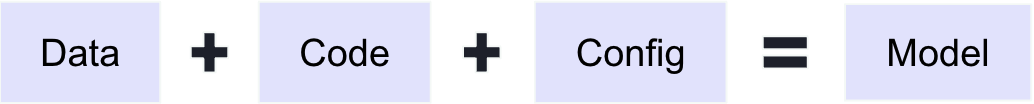
\includegraphics[width=\linewidth]{chapters/NLP/figures/model.png}
    \label{fig:model}
\end{figure}
An experiment is defined by the training code, data, and configuration.
When ML and Data Science are involved, the data generating process has to be documented.
In software engineering, code doesn't exist until it is tracked in a VCS and pushed to a remote repository.
Similarly, data doesn't exist until it is stored in a secure location, where it can be reliably retrieved, for example from a cloud storage provider, such as Dropbox, Google Drive, Amazon S3, or Google Cloud Storage.
We emphasize again the importance of having a single source of truth for all data.
In addition to the raw data, we should also store documentation about how it was created, by whom, when, and any additional processing steps.
All processing steps should be done in a way that is easy to replicate and understand -- ideally directly in code.

While VCSs are specialized to keep track of changes in plain text files, they are not well suited for tracking other aspects of an experiment.
The ML community has developed specialized tools\footnote{Weights\&Biases, Neptune}, which are excellent at tracking, visualizing and comparing of
\begin{itemize}
    \item Hyperparameters,
    \item Model metrics,
    \item (Interactive) plots,
    \item Logs,
    \item Hardware configuration,
    \item Hardware metrics,
    \item Code and dependency versions, as well as
    \item Data and Model Artifacts.
\end{itemize}
This facilitates the collaboration and sharing of results by directly linking to the experiments.

At the beginning of a new training run you should initialize an experiment tracking tool to ensure that all data related to the run is streamed to a web based platform.
For example with \texttt{Weights\&Biases} you can initialize a new experiment as follows:
\begin{python}
import wandb

wandb.init(
  project="sudep-detection",
  notes="tweak baseline",
  tags=["baseline", "paper1"],
)
\end{python}
The \pythoninline{wandb.init()} function will create a new experiment in the \texttt{sudep-detection} project, with the notes \texttt{tweak baseline} and the tags \texttt{baseline} and \texttt{paper1}.
To set and track hyperparamters we recommend using an argument parser such that we can pass in the hyperparameters as command line arguments.
Python has a built-in argument parser, \pythoninline{argparse}, which can be used as follows:
\begin{python}
import argparse
parser = argparse.ArgumentParser()
parser.add_argument(
    "--learning_rate",
    type=float,
    default=0.001,
    help="Learning rate"
)
parser.add_argument(
    "--batch_size",
    type=int,
    default=32,
    help="Batch size"
)
args = parser.parse_args()
\end{python}
The \pythoninline{argparse} module will automatically parse the command line arguments and make them available as attributes of the \pythoninline{args} object.
This also doubles as a form of documentation and validation of hyperparameters.
Next we can easily track the exact setting by using \pythoninline{wandb.config.update(args)}.

The remote platform again takes on the role of a single source of truth, making the results available to all collaborators, independently of who started the run or on which machine or service they did it.
This saves valuable time, reduces the risk of errors, and makes it easy to share results with others.
The platform will also automatically track the hardware configuration, such as the number of GPUs, CPU, RAM, and the operating system.
Once multiple experiments are tracked, the platform will allow you to compare them, for example by plotting the training loss over time, or by allowing you to filter runs by a specific tag or hyperparameter setting.

In Machine Learning, it is not uncommon to conduct hundreds of experiments until a satisfactory model and configuration is found for a given project.
Without automated and rigorous tracking, it is very easy to lose track of what you have tried and what the results were.
This is especially true when working with a team of collaborators, or when you want to build on the work of others -- or on your own work a few months later.
